\chapter[SAT Geometry]{Strategies for SAT Geometry}

\section{SAT Worksheet 1A: Warm-Up Problems}

\textbf{Strategies practice:} Draw a diagram and any information that you can described in each of the following questions

\begin{multienumerate}
\mitemxx{Points $A, B$, and $C$ are colinear and line $D$ is perpendicular to point $A$. Line $E$ is parallel to line $D$.}
{In right triangle $ABC$, point $D$ is equidistant to points $A$ and $B$ on the hypotenuse, line $AB$.}
\end{multienumerate}

\vfill
\hrulefill

\textbf{Content Practice:} The following is designed to ensure that you have a proper grasp of the concepts that you will see on the SAT math section. Read the words and definitions (if you don't already know them) and then answer the question that follows.

\bigskip
\begin{enumerate}[label=\bfseries\arabic*.]
\item \textbf{Whole Numbers, Integer, Decimal, Real Number} $-$ A whole number is any non-decimal, non-negative number (0 included). An integer is any non-decimal number, positive, negative, or 0. A decimal is a part of another number. A real number is a number that exists in the real plane instead of the imaginary.

\bigskip
\indent Identify the following numbers: $2, 0, -1, 0.25, i$

\vfill\item \textbf{Remainder} $-$ The amount left over after a long division. What is the remainder of the quotient of 20 and 2?

\vfill
\newpage
\item \textbf{Numerator/Denominator} $-$ The numerator is the number on top of a fraction. The denominator is the number on the bottom. If a fraction has a numerator of four and a denominator of five, what is its value as a decimal?

\vfill\item \textbf{Absolute Value} $-$ The distance away of a number from 0. It will always be represented as a positive number. Absolute value is represented by $|x|$.

\bigskip
\indent Evaluate the following: $|-3|+|6|\times|8|-|-15|$

\vfill\item \textbf{Sum, difference, product, quotient} $-$ The sum is the result of adding two numbers. The difference is the result of subtracting two numbers. The product is the result of multiplying two numbers. The quotient is the result of dividing two numbers.

\bigskip
\indent Find the sum, difference, product, and quotient of 15 and 5.

\vfill\item \textbf{Operation} $-$ A set of rules to explain what must the computation to be performed on two or more values

\bigskip
\indent Let the operation $x@y$ be equal to $3x+2y$. Evaluate $5@8$.

\vfill\item \textbf{Multiple, factor, prime, divisible by} $-$ A multiple is a number that can be divided by (is divisible by) another without a remainder. A factor is a number that can be used to divide another number without a remainder. A factor is anumber that can be used to divide another number without a remainder. A prime number is a number that cannot be divided by any number (except 1) without a remainder.

\bigskip
\indent List 5 multiples of 6.

\bigskip
\indent List all the positive factors of 60

\vfill\item \textbf{Consecutive} $-$ One right after another. The sum of 3 consecutive numbers is 21. What is the value of the largest number?

\vfill\item \textbf{Distinct} $-$ Different

\vfill
\newpage
\underline{Geometry Vocabulary}

\medskip
\item \textbf{Bounded} $-$ Restrained or bordered by

\bigskip
Shade in the region bound by the lines $y=2, y=2x+2$, and $y=-2x+4$ then find the three points that are the vertices of the shaded region.

\bigskip
\centerline{\begin{tikzpicture}
\draw [latex-latex] (0,2) -- (4,2) node[anchor=west] {$x$};
\draw [latex-latex] (2,0) -- (2,4) node[anchor=south] {$y$};
\draw (0,2.5) -- (3.5,2.5);
\draw (1.5,4) -- (3.5,0.5);
\draw (1.5,0.5) -- (2.5,4);
\end{tikzpicture}}

\vfill\item \textbf{Lie in a plane} $-$ Something that lies within a plane is located within the boundaries of said plane

\bigskip
State which points do an which points do not lie in plane $A$

\bigskip
\centerline{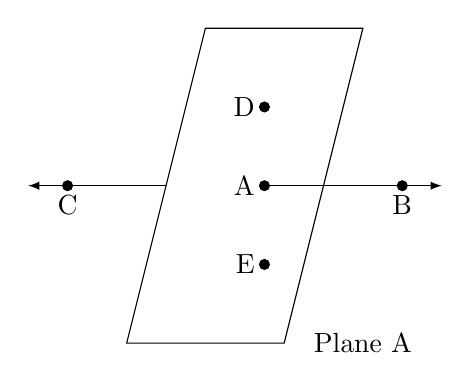
\begin{tikzpicture}
\draw (0,0) -- (2,0) -- (3,4) -- (1,4) -- cycle;
\draw [-latex] (1.75,2) -- (4,2);
\draw [latex-] (-1.25,2) -- (0.5,2);
\fill (-0.75,2) node[anchor=north] {C} circle (2pt);
\fill (3.5,2) node[anchor=north] {B} circle (2pt);
\fill (1.75,2) node[anchor=east] {A} circle (2pt);
\fill (1.75,3) node[anchor=east] {D} circle (2pt);
\fill (1.75,1) node[anchor=east] {E} circle (2pt);
\draw (3,0) node {Plane A};
\end{tikzpicture}}

\vfill\item \textbf{Acute, Right, Obtuse} $-$ An acute angle is less than 90 degrees. A right angle is exactly 90 degrees. An obtuse angle is larger than 90 degrees.

\bigskip
Identify the type of angle:

\begin{center}
\begin{multicols}{3}
\begin{tikzpicture}
\draw (0,2) -- (2,0) -- (4,0);
\draw (2,-0.5) node {A};
\end{tikzpicture}


\columnbreak
\begin{tikzpicture}
\draw (3,2) -- (0,0) -- (4,0);
\draw (2,-0.5) node {B};
\end{tikzpicture}


\columnbreak
\begin{tikzpicture}
\draw (0,2) -- (0,0) -- (2,0);
\draw (0,0.5) -- (0.5,0.5) -- (0.5,0);
\draw (1,-0.5) node {C};
\end{tikzpicture}
\end{multicols}
\end{center}

\vfill
\newpage
\item \textbf{Equilateral, Isosceles, Scalene} $-$ An equilateral triangle has three equal sides. An isosceles triangle has two equal sides. A scalene triangle has no equal sides.

Identify the type of triangle:

\begin{multicols}{3}
\begin{center}
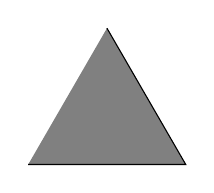
\begin{tikzpicture}
\draw[fill=gray] (0,0) -- (2,0) -- (1,1.73);
\draw (0,0);
\end{tikzpicture}

A
\end{center}

\columnbreak
\begin{center}
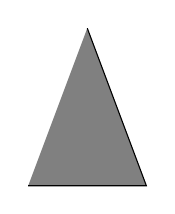
\begin{tikzpicture}
\draw[fill=gray] (0,0) -- (1.5,0) -- (0.75,2);
\end{tikzpicture}

B
\end{center}

\columnbreak
\begin{center}
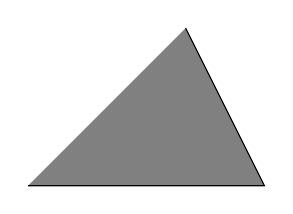
\begin{tikzpicture}
\draw[fill=gray] (0,0) -- (3,0) -- (2,2);
\end{tikzpicture}

C
\end{center}
\end{multicols}

\vfill\item \textbf{Shaded region} $-$ The area of the figure with a dark gray coloring

\bigskip
Find the area of the shaded region within the square

\begin{center}
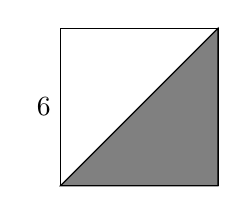
\begin{tikzpicture}
\draw (0,0) -- (2,0) -- (2,2) -- (0,2) -- cycle;
\draw[fill=gray] (0,0) -- (2,0) -- (2,2) -- cycle;
\draw (0,1) node[anchor=east] {6};
\end{tikzpicture}
\end{center}

\vfill\item \textbf{Parallel} $-$ Two lines that never intersect

\bigskip
Give an example of an equation of the line that is parallel to $y=3x+7$

\begin{center}
\begin{tikzpicture}
\draw (0,0) -- (2,2);
\draw (1,0) -- (3,2);
\end{tikzpicture}
\end{center}

\vfill\item \textbf{Perpendicular} $-$ Two lines that intersect to form a right angle

\bigskip
White two lines below are perpendicular? \underline{\hspace{1in}}

\bigskip
\centerline{\begin{tikzpicture}
\draw (0,2) node[anchor=east] {C} -- (4,2) node[anchor=west] {D};
\draw (0,3) node[anchor=south] {A} -- (3,0) node[anchor=north] {B};
\draw (2,0) node[anchor=north] {F} -- (2,4) node[anchor=south] {E};
\draw (2, 2.5) -- (2.5,2.5) -- (2.5,2);
\end{tikzpicture}}

\vfill\item \textbf{Tangent} $-$ A line that intersects at exactly one point on a circle

\bigskip
Which line is tangent to circle $R$?

\begin{center}
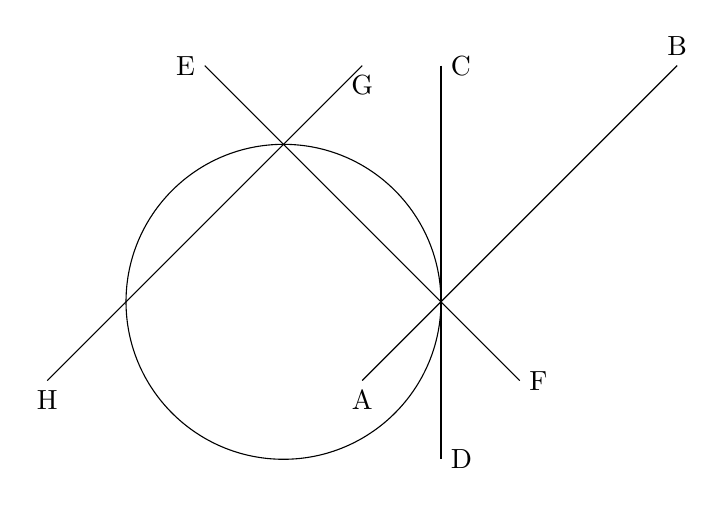
\begin{tikzpicture}
\draw (3,3) circle (2cm);
\draw (0,2) node[anchor=north] {H} -- (4,6) node[anchor=north] {G};
\draw (5,6) node[anchor=west] {C} -- (5,1) node[anchor=west] {D};
\draw (4,2) node[anchor=north] {A} -- (8,6) node[anchor=south] {B};
\draw (2,6) node[anchor=east] {E} -- (6,2) node[anchor=west] {F};
\end{tikzpicture}
\end{center}
\end{enumerate}

\vfill
\newpage
\section[General Strategies]{General Strategies for the SAT Geometry Section}

\bigskip
\textbf{Strategy \#1: Visualization is key!} As we saw in the strategy section of the warm-up, \longline can help to break up complex language and also to give you a jumping off point to start solving the problem. If the SAT problems give you a diagram as part of the problem, then you should always start by marking the information given or that you can directly deduce directly onto the image.

\bigskip
\textbf{Strategy \#2: Minimize the number of variables!} Not having numbers at the onset of a problem can increase the difficulty level of the SAT problem, particularly the geometry problems. Therefore, if you can covert these relationships or variables to \underline{\hspace{1.5in}}, then it is easier to think about and solve the problem.

\bigskip
One way to do this: Whenever there is a relationship between two objects (angles, line segments, etc.), you are probably going to need to numerically solve for this relationship. This will either be your answer or it will directly be used to find your answer. Therefore, if you see a ratio in the problem, then convert it to variables and solve for the variables if possible. If you can convert a line segment to a number line with numerical distances, then do it!

\vfill
\newpage
\section{Distances on a Line}

\bigskip
Examples:

\begin{multicols}{2}
\begin{enumerate}[label*=\arabic*.]
\item \textbf{Medium}

In the $xy$-coordinate plane, point $A$ is at $(1,5)$ and point $B$ is at $(-a,-3)$. The distance between points $A$ and $B$ is 12. What is the value of $a$?
\vfill
\phantom{}
\columnbreak
\item \textbf{Medium}

Lines $l, m,$ and $r$ are all different lines that lie in the same plane. If $l\perp m, m\perp r$, and $r\perp s$, which of the following must be true?

\bigskip
\begin{enumerate}[label=\Roman*.]
\item $l\perp s$
\item $l\parallel r$
\item $m\perp s$
\end{enumerate}

\begin{enumerate}[label=(\Alph*)]
\item I only
\item I and II only
\item I and III only
\item II and III only
\item I, II, and III
\end{enumerate}
\end{enumerate}
\end{multicols}

\vfill
Problem solving strategy for distances on a line:

\begin{spacing}{1.5}
\begin{enumerate}[label=\Roman*)]
\item \longline if one doesn't exist
\item \longline the diagram (what is equal to what, etc). Convert it to a

\longline if possible
\item Solve for the \longline of the different segments
\item Use the information in steps \#$1-3$ to \longline
\end{enumerate}
\end{spacing}

\vfill
\newpage
\section{SAT Worksheet 2A: 6, Questions, 8 Minutes}


\begin{multienumerate}
\mitemxx{\basic

\begin{center}
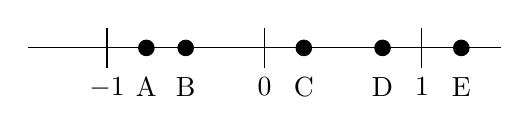
\begin{tikzpicture}
\draw (0,1) -- (6,1);
\draw (1,1.25) -- (1,0.75) node[anchor=north] {$-1$};
\fill (1.5,1) circle(3pt);
\draw (1.5,0.75) node[anchor=north] {A};
\fill (2,1) circle(3pt);
\draw (2,0.75) node[anchor=north] {B};
\draw (3,1.25) -- (3,0.75) node[anchor=north] {0};
\fill (3.5,1) circle(3pt);
\draw (3.5,0.75) node[anchor=north] {C};
\fill (4.5,1) circle(3pt);
\draw (4.5,0.75) node[anchor=north] {D};
\draw (5,1.25) -- (5,0.75) node[anchor=north] {1};
\fill (5.5,1) circle(3pt);
\draw (5.5,0.75) node[anchor=north] {E};
\end{tikzpicture}
\end{center}

Given the points on the number line above, which product has the smallest value?

\begin{enumerate}[label=(\Alph*)]
\item $A\times B$
\item $A\times C$
\item $B\times D$
\item $D\times E$
\item $B\times C$
\end{enumerate}}
{\basic

Points $P, Q, R,$ and $S$ lie on a line, in that order, so that $Q$ is the midpoint of $PR$, $R$ is the midpoint of $QS$, and $PS=18$. If point $X$ lies between $Q$ and $R$ and $QX=4$, what is the length of $XS$?

\begin{enumerate}[label=(\Alph*)]
\item 2
\item 4
\item 6
\item 8
\item 10
\end{enumerate}}

\vfill
\mitemxx{\medium

\begin{center}
\begin{tikzpicture}
\draw (0,1) -- (6,1);
\draw (1,1.25) -- (1, 0.75) node[anchor=north] {3};
\draw (2,1.25) -- (2, 0.75) node[anchor=north] {$x$};
\draw (3,1.25) -- (3, 0.75) node[anchor=north] {$y$};
\draw (4,1.25) -- (4, 0.75);
\draw (5,1.25) -- (5, 0.75) node[anchor=north] {$2x$};
\end{tikzpicture}
\end{center}

In the number line above, the tick marks are equally spaced. What is the value of $y$?

\begin{enumerate}[label=(\Alph*)]
\item 5
\item 6
\item 7
\item 8
\item 9
\end{enumerate}}
{\medium

Points $X$ and $Y$ are two different points on a circle. Point $m$ is localed so that line segment $XM$ and line segment $YM$ have equal lengths. Which of the following could be true?

\begin{enumerate}[label=\Roman*.]
\item $M$ is on the center of the circle
\item $M$ is on the arc $XY$
\item $M$ is outside of the circle
\end{enumerate}

\begin{enumerate}[label=(\Alph*)]
\item I only
\item II only
\item I and II only
\item II and III only
\item I, II, and III
\end{enumerate}}

\vfill
\mitemxx{\advanced

$R$ is the midpoint of line segment $PT$ and $Q$ is the midpoint of line segment $PR$. If $S$ is a point between $R$ and $T$ such that the length of segment $QS$ is 10 and the length of segment $PS$ is 19, what is th length of $ST$?}
{\advanced

Point $M$ is the midpoint of line segment $AB$. Points $C$ and $D$ are located on $AB$ in such a way that $AC=CM$ and $MD=DB$. If $MD=5$, what is the length of $AD$?}
\end{multienumerate}

\vfill
\newpage
\section{Angles and Lines}

\bigskip
Examples:

\begin{multienumerate}
\mitemxx{\basic

\begin{center}
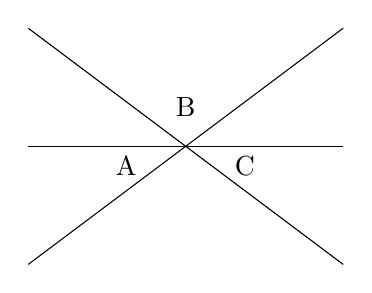
\begin{tikzpicture}
\draw (0,1.5) -- (4,1.5);
\draw (0,0) -- (4,3);
\draw (0,3) -- (4,0);
\draw (1.5,1.5) node[anchor=north east] {A};
\draw (2, 2) node {B};
\draw (2.5, 1.5) node[anchor=north west] {C};
\end{tikzpicture}
\end{center}

\bigskip
In the figure above, if $\angle A=50^\circ, \angle B=42^\circ$, and $\angle C=2x^\circ$, what is the measure of $\angle C$?

\begin{enumerate}[label=(\Alph*)]
\item $166^\circ$
\item $43^\circ$
\item $88^\circ$
\item $50^\circ$
\item $138^\circ$
\end{enumerate}
}{\medium

In the $xy$-plane, line $l$ is $2x-3y=5$. Which of the following coordinates are on a line perpendicular to line $l$ with a $y$-intercept of $-10$?

\begin{enumerate}[label=(\Alph*)]
\item $(-2,4)$
\item $(-6,-1)$
\item $(-6,-2)$
\item $(-2,-7)$
\item $(-1,-4.5)$
\end{enumerate}}
\end{multienumerate}

\hrulefill

What is the sum of angles of a straight line?

\begin{center}
\begin{tikzpicture}
\draw (0,0) -- (4,0);
\draw (1,0) -- (4,2);
\draw[color=red] (1.5,0) arc (0:180:0.5);
\end{tikzpicture}
\end{center}

What is the sum of angles around two straight lines? In this case, which angles are congruent? Why?

\begin{center}
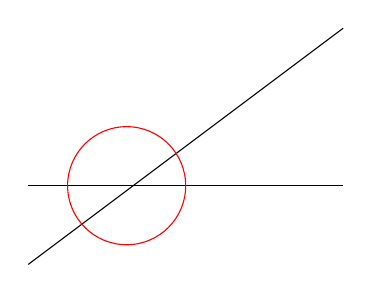
\begin{tikzpicture}
\draw (0,0) -- (4,0);
\draw (0,-1) -- (4,2);
\draw[color=red] (2,0) arc (0:360:0.75);
\end{tikzpicture}
\end{center}

In the figure to the right, lines $l$ and $m$ are parallel. Which angles or sums of angles are congruent? Which angles sum to $180^\circ$ and why?

\begin{center}
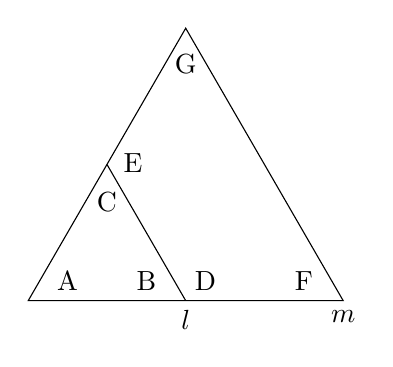
\begin{tikzpicture}
\draw (0,0) -- (4,0) node[anchor=north] {$m$} -- (2,3.46) -- cycle;
\draw (0.5,0.25) node {A};
\draw (1.5,0.25) node {B};
\draw (2.25,0.25) node {D};
\draw (3.5,0.25) node {F};
\draw (1,1.73) -- (2,0) node[anchor=north] {$l$};
\draw (1,1.25) node {C};
\draw (1.33,1.75) node {E};
\draw (2,3) node {G};
\end{tikzpicture}
\end{center}

Other questions will ask you about the slope of a line or about parallel or perpendicular lines.

\bigskip
\textbf{To find the slope of a line:} You need at least 2 points on the line. Write down the $x$ and $y$ coordinates for points 1 and 2. Then, slope = $(y_2-y_1)/(x_2-x_1)$.

\bigskip
\textbf{About parallel lines:} Parallel lines have the same slope. To find the equation of a line parallel to the given line, find the slope of the given line (see \#1). It is also the ``$m$'' term in the equation of a line, $y=mx+b$. Then, plug in $x$ and $y$ coordinates to the equation of a line with the same $m$ as the original line and solve for $b$.

\bigskip
\textbf{About perpendicular lines:} The slopes of perpendicular lines are negative reciprocals. To find the equation of a line perpendicular to a given line, Find the slope of the given line (see \#1). It is also the ``$m$'' term in the equation of a line, $y=mx+b$. Then, take it's negative reciprocal to find the slope for the perpendicular line. Plug in $x$ and $y$ coordinates to the equation of a line with the m that was solved for in the previous step. Solve for $b$.

\newpage
\subsection{SAT Worksheet 3A: 6 Questions, 8 Minutes}

\begin{multienumerate}
\mitemxx{\basic

\begin{center}
\begin{tikzpicture}
\draw (0.5,0.5) node[anchor=south] {$m$}-- (6,1.5);
\draw (0.25,2) node[anchor=south] {$l$} -- (6,3);
\draw (3,4) -- (3,0);
\draw (3,2.75) node[anchor=east] {A};
\draw (3,2.25) node[anchor=west] {B};
\draw (3,1.25) node[anchor=west] {C};
\end{tikzpicture}
\end{center}

If $l \parallel m, B=(x+5)^\circ$, and $C=(3x-17)^\circ$, what is the measurement of angle $A$?
}{\basic

\begin{tikzpicture}
\draw (0,0) -- (4,0);
\draw (2,0) node[anchor=south east] {$x$} -- (4,2);
\draw (3,0) node[anchor=south east] {$y$};
\end{tikzpicture}

In the figure above, what is $y$ in terms of $x$?

\begin{enumerate}[label=(\Alph*)]
\item $90^\circ-x$
\item $90^\circ-x/2$
\item $90^\circ+x/2$
\item $120^\circ-x$
\item $180^\circ-x$
\end{enumerate}}

\mitemxx{\medium

\begin{center}
\begin{tikzpicture}
\draw (0,2) -- (6,2);
\fill (1,2) node[anchor=south] {D} circle (2pt);
\draw[fill=black] (5,1) node[anchor=north] {C} -- (3.5,2) node[anchor=south east] {B} circle (2pt) -- (5,3) node[anchor=south] {A};
\end{tikzpicture}
\end{center}

If line A bisects $\angle ABC$, and the measure of $\angle ABC$ is $80^\circ$, what is the value of $\angle CBD$?
}{\medium

\begin{center}
\begin{tikzpicture}
\draw (0,0) -- (4,0) -- (5,2) -- (1,2) -- cycle;
\draw (3.5,0) arc (180:420:0.5);
\draw (4.5,-0.625) node {$y$};
\draw (4.5,2) arc (180:-120:0.5);
\draw (5.625,2.275) node {$x$};
\end{tikzpicture}
\end{center}

The figure above is a parallelogram. If $x=300^\circ$, what is the value of $y$?

\begin{enumerate}[label=(\Alph*)]
\item $200^\circ$
\item $240^\circ$
\item $280^\circ$
\item $320^\circ$
\item $330^\circ$
\end{enumerate}}

\mitemxx{\advanced

The measure of the largest angle in a certain triangle is twice the sum of the measures of the remaining angles. What is the measure of the largest angle?

\begin{enumerate}[label=(\Alph*)]
\item $45^\circ$
\item $60^\circ$
\item $90^\circ$
\item $120^\circ$
\item $150^\circ$
\end{enumerate}
}
{\advanced

The line in the $xy$-plane that contains the points $(2, 5)$ and $(4, y)$ has slope 0. What is the value of $y$?}
\end{multienumerate}

\newpage
\textbf{\large Triangles}

\bigskip
Examples

\begin{multienumerate}
\mitemxx{\basic

\begin{center}
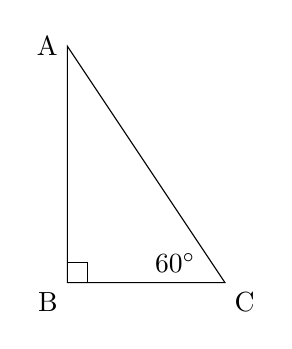
\begin{tikzpicture}
\draw (0,0) node[anchor=north east] {B} -- (2,0) node[anchor=north west] {C} -- (0,3) node[anchor=east] {A} -- cycle;
\draw (0,0.25) -- (0.25,0.25) -- (0.25,0);
\draw (1.75,0) node[anchor=south east] {$60^\circ$};
\end{tikzpicture}
\end{center}

If $AB=8$, what is the length of $AC$?
}{\medium

\begin{center}
\begin{tikzpicture}
\draw (0,0) node[anchor=north east] {B} -- (2,0) node[anchor=north west] {C} -- (0,3) node[anchor=east] {A} -- cycle;
\draw (0,0.25) -- (0.25,0.25) -- (0.25,0);
\end{tikzpicture}
\end{center}

If $AB=BC=4/11$, what is the value of $AC$? What is the value of $x$?
}
\end{multienumerate}

\hrulefill

There are two main types of questions with triangles on the SATs that involve triangles: solving for angles in a triangle and solving for a side length of a triangle. Many of these will involve special right triangles.

\bigskip
Solving for side lengths: You will primarily use the Pythagorean theorem and Pythagorean triples, rules of special right triangles, and rules of the lengths of a triangle. 

\bigskip
\begin{enumerate}[label=\arabic*)]
\item What is the general rule for the lengths of the side lengths of a triangle?
\vfill\item What are Pythagorean triples? In what types of problems can they be used on the SAT?
\vfill\item What are examples of Pythagorean triples? The most commonly used Pythagorean triples on the SAT are \longline
\vfill\item What are the rules for side lengths of $30^\circ-60^\circ-90^\circ$ special right triangles?
\vfill\item What are the rules for side lengths of $45^\circ-45^\circ-90^\circ$ special right triangles?
\end{enumerate}

\vfill
\newpage
\textbf{\large Complex Polygons}

There are many types of problems with angles in triangles and more complex shapes. Many will ask students to integrate knowledge of the types of angles (of triangles and n-shaped polygons) and straight, parallel and perpendicular lines. 

\bigskip
\begin{enumerate}[label=\arabic*)]
\item What is the general formula for the sum of the interior angles of a n-sided polygon?
\vfill\item What is the sum of the interior angles of a quadrilateral?
\vfill\item What is the sum of the interior angles of a pentagon?
\vfill\item What is the sum of the interior angles of a hexagon?
\vfill\item What is the sum of the interior angles of an octagon?
\end{enumerate}

\vfill
\section[Complex Polygons]{General Strategies for Finding Angles in a Complex Polygon}

\bigskip
\begin{enumerate}[label=\arabic*)]
\item Identify the large polygon(s) and the polygons within the main polygon. Try to fill in \longline that you do know based on the sum of interior angles of a triangle, quadrilateral, or other polygons in the problem.

\bigskip\item Try to fill in angles that you do know using properties of \longline

\bigskip\item Then try to put the information from steps 1 and 2 together to try to solve for more angles in the polygon and eventually the angle or variable that you are looking for. 
\end{enumerate}

\newpage
\subsection{SAT Worksheet 4A: 6 Questions, 8 Minutes}

\begin{multienumerate}
\mitemxx{\basic

What is the minimum possible side length for a triangle with one side length of 3 and another side length of 4? Round to the nearest hundredth.
}{\basic

\centerline{\includegraphics{12}}

All of the following are true EXCEPT

\begin{enumerate}[label=(\Alph*)]
\item $A+B+C=180^\circ$
\item $A+B+C=C+D$
\item $A+B=D$
\item $D=90^\circ$
\item $180^\circ-C=D$
\end{enumerate}}

\vfill
\mitemxx{\medium

\begin{center}
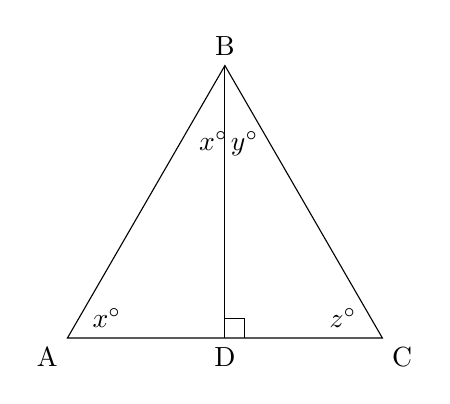
\begin{tikzpicture}
\draw (0,0) node[anchor=north east] {A} -- (4,0) node[anchor=north west] {C} -- (2,3.46) node[anchor=south] {B} -- cycle;
\draw (2,3.46) -- (2,0) node[anchor=north] {D};
\draw (2,0.25) -- (2.25,0.25) -- (2.25,0);
\draw (0.5,0.25) node {$x^\circ$};
\draw (3.5,0.25) node {$z^\circ$};
\draw (2.16,2.75) node[anchor=north east] {$x^\circ$};
\draw (2.25,2.75) node[anchor=north] {$y^\circ$};
\end{tikzpicture}
\end{center}

If $z=30^\circ$, and $BC=3/4$, what is the length of $AC$, rounded to the nearest hundredth?
}{\medium

Triangle $ABC$ has side lengths 6 and 9. Which of the following could be the length of the third side?

\begin{enumerate}[label=\Roman*.]
\item 3
\item 5
\item 15
\end{enumerate}

\begin{enumerate}[label=(\Alph*)]
\item I only
\item II only
\item III only
\item I and II only
\item I, II, and III
\end{enumerate}}

\vfill
\mitemxx{\advanced

A triangle with vertices at points $A (1,4), B(-1,4)$, and $C(7,4)$ is reflected across the $y$-axis. What is the new $y$-coordinate of point $A$?
}{\advanced

What is the largest possible difference in area between two triangles each with side lengths of 7 and 9, rounded to the nearest hundredth?}
\end{multienumerate}

\vfill

\newpage
\subsection{SAT Worksheet 5A (Basic): 6 Questions, 8 Minutes}

\begin{multienumerate}
\mitemxx{A line contains two points with coordinates $(-2,-3)$ and $(7,10)$. Which of the following points are also on the line?

\begin{enumerate}[label=(\Alph*)]
\item $(4,2)$
\item $(9,12)$
\item $(6,5)$
\item $(5,-6)$
\item $(16,23)$
\end{enumerate}
}{A right triangle has a hypotenuse of length 26 and one leg of length 24. What is 200\% of the length of the other leg?

\begin{enumerate}[label=(\Alph*)]
\item 5
\item 10
\item 12
\item 20
\item 24
\end{enumerate}
}

\vfill
\mitemxx{

\medskip
\centerline{\includegraphics{14}}

Line $l$ has a slope of $-2$ and a $y$-intercept of 2. What is the $x$-intercept of line $l$?

\begin{enumerate}[label=(\Alph*)]
\item $-1$
\item 2
\item 1
\item 4
\item $-2$
\end{enumerate}
}{Points $P, Q$, and $R$ are collinear and graphed on the $xy$ coordinate plane. $R$ is the midpoint of points $P$ and $Q$. $PS$ is the same length as $PR$. Which of the following are plausible?

\begin{enumerate}[label=\Roman*.]
\item Point $S$ has the same coordinates as point $P$
\item $PQ$ is perpendicular to $RS$
\item $PS>PQ$
\end{enumerate}

\begin{enumerate}[label=(\Alph*)]
\item I only
\item II only
\item I and II only
\item I, II, and III
\item None of the above
\end{enumerate}
}

\vfill
\mitemxx{If square $ABCD$ has an area of 5, what is the length of diagonal $AC$?

\begin{enumerate}[label=(\Alph*)]
\item 5
\item $5\sqrt2$
\item 10
\item $10\sqrt2$
\item $\sqrt10$
\end{enumerate}}
{Which of the following equations of lines has a positive slope and has a possible solution of $(3,5)$?

\begin{enumerate}[label=(\Alph*)]
\item $y+3x=5$
\item $-2x+y= -1$
\item $y=2x-10$
\item $x^2-6=y$
\item $2(x+y)=5$
\end{enumerate}}
\end{multienumerate}

\newpage
\subsection{SAT Worksheet 6A (Medium): 6 Questions, 9 Minutes}

\begin{multienumerate}
\mitemxx{

A scalene triangle has side lengths that are each an integer. If the hypotenuse of the triangle is 5, what is the largest possible absolute value difference between the shortest leg and longest leg to the nearest hundredth?

\begin{enumerate}[label=(\Alph*)]
\item 3.00
\item 4.00
\item 1.00
\item 10.00
\item $\sqrt10$
\end{enumerate}
}{

\smallskip
\centerline{\includegraphics{15}}

\begin{center}
\begin{tikzpicture}
\draw (3,4) -- (0,0) -- (4,0) -- (2,2.66) node[anchor=west] {$(3b)^\circ$};
\end{tikzpicture}
\end{center}

Which of the following expressions can be demonstrated by the figure above?

\begin{enumerate}[label=(\Alph*)]
\item $(a-23)^\circ=3b$
\item $(2a-43)^\circ+(-a+20)^\circ>(3b)^\circ$
\item $(2a-43)^\circ=(-a+20)^\circ$
\item $a=(3b)^\circ20$
\item $a-23>(3b)^\circ$
\end{enumerate}
}

\vfill
\mitemxx{In the $xy$-plane, the points with coordinates $(0,1)$ and $(4,t)$ lie on line $l$. If the slope of l is greater than $1/4$ but less than $1/2$, what is one possible value of $t$?

\begin{enumerate}[label=(\Alph*)]
\item 0
\item 1
\item 1.5
\item 2
\item 2.5
\end{enumerate}
}{On a $xy$-plane, line $l$ is perpendicular to the $x$-axis and is 3 units from the $y$-axis. Which of the following points could be on line $l$?

\begin{enumerate}[label=(\Alph*)]
\item $(1,3)$
\item $(3,5)$
\item $(0,3)$
\item $(2,1)$
\item $(1,2)$
\end{enumerate}}

\vfill
\mitemxx{If a circle has an area of $h\pi$, what is the diameter of the circle?

\begin{enumerate}[label=(\Alph*)]
\item $(2h)^2$
\item $h$
\item $2\sqrt h$
\item $h^2$
\item $\sqrt{h}/2$
\end{enumerate}}
{A circle and a triangle are coplanar. What are the maximum number of intersection points between the two shapes?

\begin{enumerate}[label=(\Alph*)]
\item 3
\item 4
\item 5
\item 6
\item More than 6
\end{enumerate}}
\end{multienumerate}

\newpage
\subsection{SAT Worksheet 7A (Advanced): 6 Questions, 10 Minutes}

\begin{multienumerate}
\mitemxx{The equation $tx+12y=-3$ is the equation of a line in the $xy$-plane, and t is a constant. If the slope of the line is $-10$, what is the value of $t$?}{On an $xy$-plane, Point R has coordinates $(0,r)$ and Point $S$ has coordinates $(s,0)$. What is the slope of line $l$?

\begin{enumerate}[label=(\Alph*)]
\item $-r/s$
\item $r/s$
\item $-s/r$
\item $s/r$
\item $-1/rs$
\end{enumerate}}

\vfill
\mitemxx{Point $A$ has coordinates $(a,b)$ and is in the fourth quadrant. Point $B$ is in the third quadrant. Points $A$ and $B$ are the same distant from the origin. Which of the following could be the coordinates of point $B$?

\begin{enumerate}[label=(\Alph*)]
\item $(-a,b)$
\item $(a,b)$
\item $(-b,-a)$
\item $(-b,a)$
\item $(b,a)$
\end{enumerate}}
{Points on the line $2x+y=1$ lie in which of the following sets of quadrants?

\begin{enumerate}[label=(\Alph*)]
\item I and III only
\item I and IV only
\item I, II, and III
\item I, II and IV
\item I, III, and IV
\end{enumerate}}

\vfill
\mitemxx{In the quadrilateral $ABCD$, point $E$ is on the line segment $AB$. The ratio of $AE$ to $EB$ is $5:4$. $AE=BC=2$. What is the area of the triangle $EBC$?}
{If a cube has an edge of 3, what is the maximum distance from one vertex to another, rounded to the nearest hundredth?}
\end{multienumerate}

\vfill
\pagebreak